\documentclass{article} 
\usepackage{polski} %moze wymagac dokonfigurowania latexa, ale jest lepszy niż standardowy babel'owy [polish] 
\usepackage[utf8]{inputenc} 
\usepackage[OT4]{fontenc} 
\usepackage{graphicx,color} %include pdf's (and png's for raster graphics... avoid raster graphics!) 
\usepackage{url} 


% Zmiana rozmiarów strony tekstu
\addtolength{\voffset}{-1cm}
\addtolength{\hoffset}{-1cm}
\addtolength{\textwidth}{2cm}
\addtolength{\textheight}{2cm}

%bardziej zyciowe parametry sterujace rozmieszczeniem rysunkow
\renewcommand{\topfraction}{.85}
\renewcommand{\bottomfraction}{.7}
\renewcommand{\textfraction}{.15}
\renewcommand{\floatpagefraction}{.66}
\renewcommand{\dbltopfraction}{.66}
\renewcommand{\dblfloatpagefraction}{.66}
\setcounter{topnumber}{9}
\setcounter{bottomnumber}{9}
\setcounter{totalnumber}{20}
\setcounter{dbltopnumber}{9}

% własny bullet list z malymi odstepami
\newenvironment{tightlist}{
\begin{itemize}
  \setlength{\itemsep}{1pt}
  \setlength{\parskip}{0pt}
  \setlength{\parsep}{0pt}}
{\end{itemize}}

%obrazkow szukamy w nastepujacym katalogu:
\graphicspath{{pics/}}



%\title{Sprawozdanie z laboratorium:\\Metaheurystyki i Obliczenia Inspirowane Biologicznie}
%\author{}
%\date{}

\begin{document}

\thispagestyle{empty} %bez numeru strony

\begin{center}
{\large{Sprawozdanie z laboratorium:\\
Bioinformatyka\\
(szablon)}}

\vspace{3ex}

Część I: Analiza teoretyczna
%Część II: Algorytmy optymalizacji lokalnej i globalnej, problem QAP
%Część III: Eksperyment: ... (prezentację można zrobić w LaTeX - służy do tego klasa "beamer")

\vspace{3ex}
{\footnotesize\today}

\end{center}


\vspace{10ex}

Prowadzący: prof. dr hab.~inż. Marta Kasprzak

\vspace{5ex}

Autorzy:
\begin{tabular}{lllr}
\textbf{Damian Jurga} & inf..... & I2 & jasiu@serwer.domena.poczta.pl \\
\textbf{Grzegorz Miebs} & inf122453 & I2 & grzegorz.miebs@student.put.poznan.pl \\
\end{tabular}

\vspace{5ex}

Zajęcia środowe, 11:45.

\vspace{35ex}

\noindent Oświadczamy, że niniejsze sprawozdanie zostało przygotowane wyłącznie przez powyższych autorów,
a wszystkie elementy pochodzące z innych źródeł zostały odpowiednio zaznaczone i~są cytowane w bibliografii.  

\newpage



\section{Wstęp}
Celem tego sprawozdania jest przedstawienie opracowania metody heurystycznej rozwiązującej problem sekwencjonowania łańcuchów DNA z błędami pozytywnymi oraz negatywnymi w czasie wielomianowym. Algorytm mając dany na wejściu zbiór oligonukleotydów (tj. ciągów nukleotydów: adeniny, tyminy, guaniny i cytozyny), długość sekwencji oryginalnej, powinien zwrócić jak najdłuższą sekwencję.

W tym celu zaproponowano następujący algorytm: sekwencja jest budowana za pomocą algorytmu wiązkowego, następnie poprawiana algorytmem wspinaczkowym i, jeżeli to możliwe, ponownie przedłużana algorytmem wiązkowym lub poprzez pełny przegląd. Przyjęto szerokość wiązki równą osiem, maksymalną liczbę iteracji algorytmu wspinaczkowego  równą sto oraz karę za ponowne odwiedzenie tego samego wierzchołku równą pięć.

\section{Wyniki}

Pomiarów dokonano na procesorze intel i7, 4 rdzeniowym, taktowowanym z częstotliwością 3 GHz.
Mierzono czas wykonania, długość sekwencji oraz liczbę wykorzystanych oligonukleotydów.
Wyniki porównano według długości sekwencji wyjściowej (liczby nukleotydów), liczby wykorzystanych oligonukleotydów oraz czasu wykonania.
Porównywano w funkcjach mocy wejściowego zbioru oligonukleotydów oraz długości nici kwasu nukleinowego, który posłużył do jego utworzenia.


\subsection{Wszystkie instancje}

\begin{figure}[h]
\makebox[\textwidth][c]{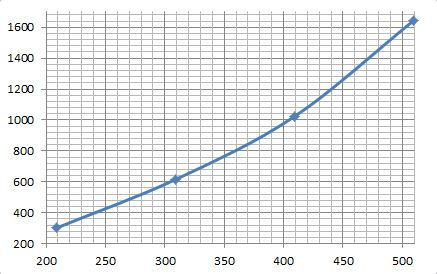
\includegraphics[scale=1]{mt(n).jpg}}
\caption{\textit{Na osi odciętych odłożona jest długość sekwencji wejściowej, a na rzędnych --- czas wykonywania w milisekundach}}
\end{figure}

\begin{figure}[h]
\makebox[\textwidth][c]{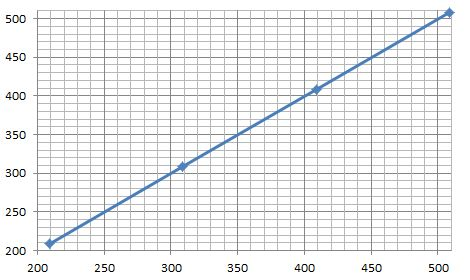
\includegraphics[scale=1]{mn(n).jpg}}
\caption{\textit{Na osi odciętych odłożona jest długość sekwencji wejściowej, a na rzędnych --- długość sekwencji wyjściowej}}
\end{figure}

Czas wykonania, jak widać na rysunku 1. jest funkcją wielomianową; można ją przybliżyć następującym dwumianem długości kwasu nukleinowego: $0.0076n^2-1.0704n+198.69$.
Długość sekwencji wyjściowej na rys.2. jest w przybliżeniu równa długości sekwencji wejściowej ($n_{out} = 0.99n_{in}-0.16$).
Rozważanie wartości w funkcji mocy zbioru nie ma sensu, gdyż w większości przypadków wartość funkcji sprowadzałaby się do wartości funkcji obliczanych dla jednej z typów instancji.

\subsection{Porównanie poszczególnych typów instancji}

\subsubsection{Według czasu}

\begin{figure}[!htbp]
\makebox[\textwidth][c]{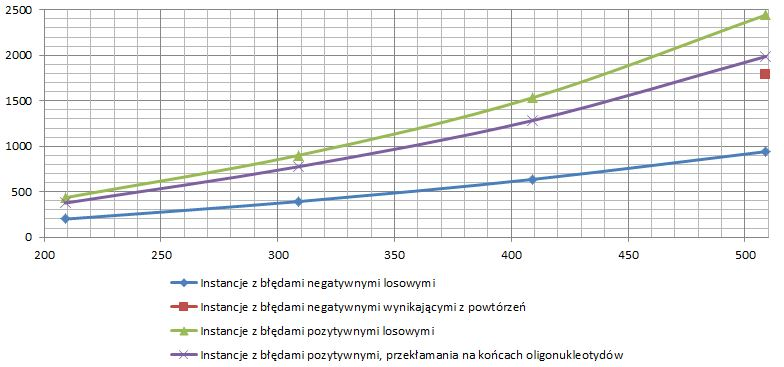
\includegraphics[scale=0.75]{t(n).jpg}}
\caption{\textit{Na osi odciętych odłożona jest długość sekwencji wejściowej, a na rzędnych --- czas wykonywania w milisekundach}}
\end{figure}

\begin{figure}[!htbp]
\makebox[\textwidth][c]{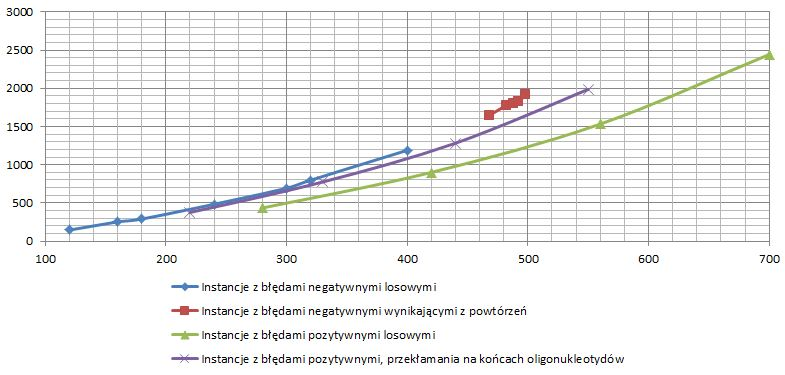
\includegraphics[scale=0.75]{t(S).jpg}}
\caption{\textit{Na osi odciętych odłożona jest moc zbioru oligonukleotydów, a na rzędnych --- czas wykonywania w milisekundach}}
\end{figure}

Jak widać na rys.3., szybciej zostały wykonane obliczenia dla instancji z błędami negatywnymi o tych samych docelowych długościach.
Wynika to zapewne z konieczności zbadania mniejszej liczby ślepych odnóg algorytmu wiązkowego.

Na rys.4. widać, że instancje z błędami pozytywnymi były wykonywane wolniej dla zbiorów o podobnej mocy.
W przypadku instancji o błędach negatywnych, czas wykonywania nie wydaje się zależeć w znaczącym stopniu od tego, czy wynikają z powtórzeń, czy są w pełni losowe.
Ten wykres każe podejrzewać, że w badanym zakresie znaczący wpływ na czas wykonywania ma przede wszystkim moc zbioru oligonukleotydów, a więc i liczba błędów.

Oba wykresy sugerują, że przyjęty algorytm ma złożoność wielomianową, zgodnie z wcześniejszą analizą teoretyczną.

\subsubsection{Według długości sekwencji wyjściowej}


\begin{figure}[!htbp]
\makebox[\textwidth][c]{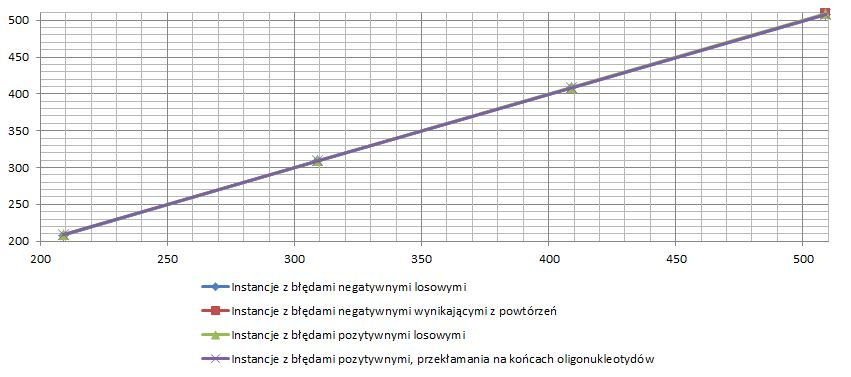
\includegraphics[scale=0.75]{n(n).jpg}}
\caption{\textit{Na osi odciętych odłożona jest długość sekwencji wejściowej, a na rzędnych --- długość sekwencji wyjściowej}}
\end{figure}

\begin{figure}[!htbp]
\makebox[\textwidth][c]{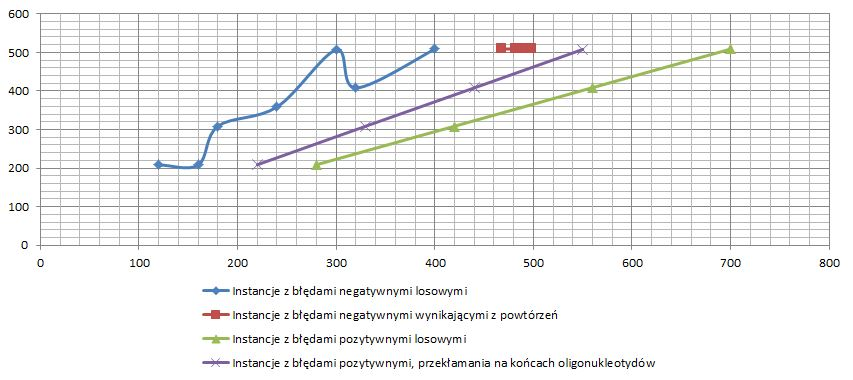
\includegraphics[scale=0.75]{n(S).jpg}}
\caption{\textit{Na osi odciętych odłożona jest moc zbioru oligonukleotydów, a na rzędnych --- długość sekwencji wyjściowej}}
\end{figure}

Rys.5. wydaje się potwierdzać skuteczność algorytmu --- sekwencje wyjściowe, dla każdego typu instancji, osiągają długość bardzo bliską docelowej.

Jak widać na rys.6. instancje z błędami pozytywnymi zależą liniowo od mocy zbioru.
W przypadku instancji z błędami negatywnymi liczba błędów jest tak duża, że powoduje ''przeskok do niższej kategorii'' i tak, na przykład przypadek, który ma osiągnąć długość 500 na wejściu zadaje zbiór o mocy mniejszej niż taki, który ma osiągnąć długość 400, przez co charakter funkcji nie jest widoczny.

\subsubsection{Według liczby wykorzystanych nukleotydów}

\begin{figure}[!htbp]
\makebox[\textwidth][c]{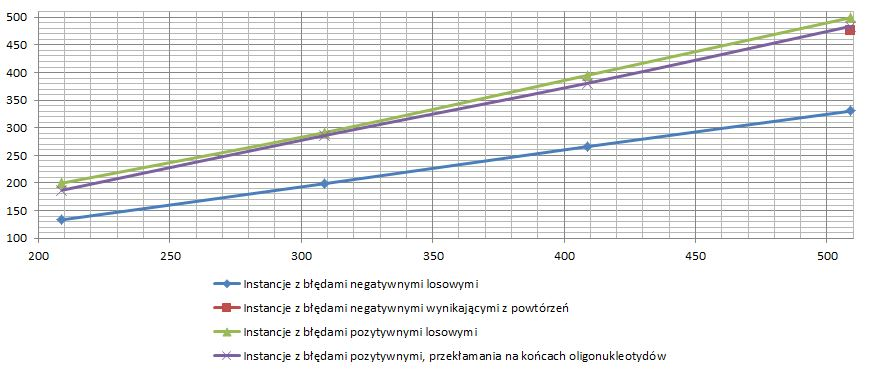
\includegraphics[scale=0.75]{i(n).jpg}}
\caption{\textit{Na osi odciętych odłożona jest długość sekwencji wejściowej, a na rzędnych --- liczba wykorzystanych oligonukleotydów (bez powtórzeń)}}
\end{figure}

\begin{figure}[!htbp]
\makebox[\textwidth][c]{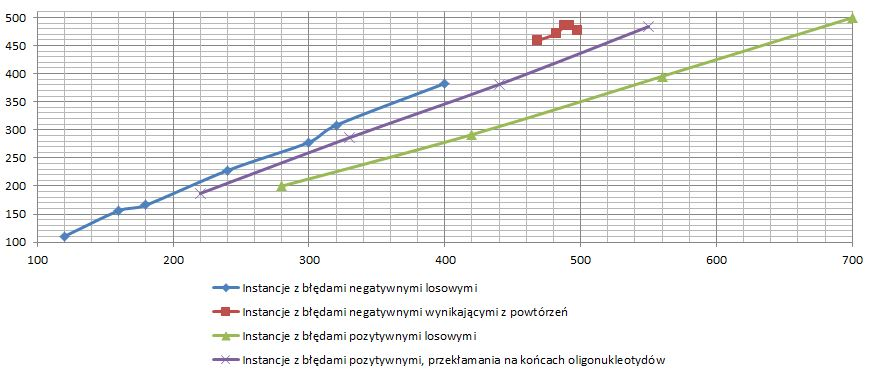
\includegraphics[scale=0.75]{i(S).jpg}}
\caption{\textit{Na osi odciętych odłożona jest moc zbioru oligonukleotydów, a na rzędnych --- liczba wykorzystanych oligonukleotydów (bez powtórzeń)}}
\end{figure}

Rys.7. obrazuje oczywistą zależność, że liczba wykorzystanych oligonukleotydów zależy liniowo od docelowej długości łańcucha, który zostanie z nich zbudowany.
Wszystkie funkcje przedstawione na rys.8. są w przybliżeniu prostymi. 
Widać, że błędy negatywne leżą niemalże na tej samej prostej, a więc można podejrzewać, że umiejscowienie błędu nie wpływa w zadanym zakresie na wynik.
Ta prosta ma współczynnik kierunkowy bliski jeden, gdyż obecność błędów negatywnych nie przeszkadza zmusza do wykorzystania jak największej liczby oligonukleotydów.
Proste odpowiadające instancjom z błędami pozytywnymi  mają niższy współczynnik kierunkowy, gdyż błędy pozytywne wymuszają z drugiej strony nie wykorzystywanie pewnych oligonukleotydów.

\section{Wyniki ujęte w tabeli}

Jak widać w tabelach 1-4 instancje z błędami negatywnymi wykorzystują średnio 95\% swoich oligonukleotydów, a te z błędami pozytywnymi 78\%, co zgadza się z charakterem wcześniej omówionych wykresów.
W instancjach z błędami negatywnymi przeskakiwane jest średnio 98 nukleotydów, a z pozytywnymi --- 8, ale rozważając jedynie te zawierające tylko błędy losowe średnie liczby skoków stają się odpowiednio 115 i 3.

\begin{table}
\caption{Instancje z błędami negatywnymi wynikającymi z powtórzeń}
\makebox[\textwidth][c]{
\begin{tabular}{|c|c|c|c|c|c|c|c|c|c|}
\hline
lp	&	ilość	&	l	&	n	&	czas[ms]	&	użyte	&	użyte	&	długość &	procent	&	skoki	\\
& nukleotydów &&&& oligonukleotydy & oligonukleotydy & wynikowa & użytych &\\
&&&&&(z powtórzeniami)&&&&\\\hline
24	&	498	&	10	&	509	&	1913	&	487	&	477	&	509	&	95	&	13	\\\hline
25	&	492	&	10	&	509	&	1828	&	492	&	486	&	509	&	98	&	8	\\\hline
26	&	488	&	10	&	509	&	1795	&	488	&	486	&	509	&	99	&	12	\\\hline
27	&	482	&	10	&	509	&	1775	&	478	&	471	&	509	&	97	&	22	\\\hline
28	&	468	&	10	&	509	&	1646	&	464	&	459	&	509	&	98	&	36	\\\hline
\end{tabular}
}
\end{table}


\begin{table}
\caption{Instancje z błędami pozytywnymi losowymi	Instancje z błędami pozytywnymi, przekłamania na końcach oligonukleotydów
}
\makebox[\textwidth][c]{
\begin{tabular}{|c|c|c|c|c|c|c|c|c|c|}
\hline
lp	&	ilość	&	l	&	n	&	czas[ms]	&	użyte	&	użyte	&	długość &	procent	&	skoki	\\
& nukleotydów &&&& oligonukleotydy & oligonukleotydy & wynikowa & użytych &\\
&&&&&(z powtórzeniami)&&&&\\\hline
29	&	280	&	10	&	209	&	445	&	200	&	200	&	209	&	71	&	0	\\\hline
30	&	280	&	10	&	209	&	434	&	200	&	200	&	209	&	71	&	0	\\\hline
31	&	280	&	10	&	209	&	428	&	200	&	200	&	209	&	71	&	0	\\\hline
32	&	420	&	10	&	309	&	923	&	295	&	295	&	309	&	70	&	5	\\\hline
33	&	420	&	10	&	309	&	896	&	281	&	280	&	309	&	66	&	19	\\\hline
34	&	420	&	10	&	309	&	886	&	300	&	300	&	309	&	71	&	0	\\\hline
35	&	560	&	10	&	409	&	1515	&	400	&	400	&	409	&	71	&	0	\\\hline
36	&	560	&	10	&	409	&	1557	&	400	&	400	&	409	&	71	&	0	\\\hline
37	&	560	&	10	&	409	&	1530	&	386	&	386	&	409	&	68	&	14	\\\hline
38	&	700	&	10	&	509	&	2470	&	500	&	500	&	509	&	71	&	0	\\\hline
39	&	700	&	10	&	509	&	2461	&	500	&	500	&	509	&	71	&	0	\\\hline
40	&	700	&	10	&	509	&	2402	&	499	&	499	&	509	&	71	&	1	\\\hline
\end{tabular}
}
\end{table}


\begin{table}
\caption{Instancje z błędami pozytywnymi, przekłamania na końcach oligonukleotydów}
\makebox[\textwidth][c]{
\begin{tabular}{|c|c|c|c|c|c|c|c|c|c|}
\hline
lp	&	ilość	&	l	&	n	&	czas[ms]	&	użyte	&	użyte	&	długość &	procent	&	skoki	\\
& nukleotydów &&&& oligonukleotydy & oligonukleotydy & wynikowa & użytych &\\
&&&&&(z powtórzeniami)&&&&\\\hline
41	&	220	&	10	&	209	&	350	&	178	&	171	&	209	&	77	&	22	\\\hline
42	&	220	&	10	&	209	&	389	&	199	&	199	&	209	&	90	&	1	\\\hline
43	&	220	&	10	&	209	&	391	&	194	&	191	&	209	&	86	&	6	\\\hline
44	&	330	&	10	&	309	&	784	&	292	&	290	&	309	&	87	&	8	\\\hline
45	&	330	&	10	&	309	&	753	&	286	&	278	&	309	&	84	&	14	\\\hline
46	&	330	&	10	&	309	&	792	&	291	&	291	&	309	&	88	&	9	\\\hline
47	&	440	&	10	&	409	&	1280	&	381	&	380	&	407	&	86	&	19	\\\hline
48	&	440	&	10	&	409	&	1333	&	385	&	385	&	409	&	87	&	15	\\\hline
49	&	440	&	10	&	409	&	1237	&	382	&	378	&	409	&	85	&	18	\\\hline
50	&	550	&	10	&	509	&	1990	&	489	&	489	&	509	&	88	&	11	\\\hline
51	&	550	&	10	&	509	&	2076	&	483	&	483	&	506	&	87	&	17	\\\hline
52	&	550	&	10	&	509	&	1898	&	485	&	480	&	509	&	87	&	15	\\\hline
\end{tabular}
}
\end{table}

\begin{table}[!htbp]
\caption{Instancje z błędami negatywnymi losowymi}
\makebox[\textwidth][c]{
\begin{tabular}{|c|c|c|c|c|c|c|c|c|c|}
\hline
lp	&	ilość	&	l	&	n	&	czas[ms]	&	użyte	&	użyte	&	długość &	procent	&	skoki	\\
& nukleotydów &&&& oligonukleotydy & oligonukleotydy & wynikowa & użytych &\\
&&&&&(z powtórzeniami)&&&&\\\hline
0	&	160	&	10	&	209	&	267	&	160	&	160	&	207	&	100	&	40	\\\hline
1	&	120	&	10	&	209	&	166	&	120	&	120	&	207	&	100	&	80	\\\hline
2	&	160	&	10	&	209	&	249	&	155	&	155	&	209	&	96	&	45	\\\hline
3	&	120	&	10	&	209	&	132	&	106	&	105	&	209	&	87	&	94	\\\hline
4	&	160	&	10	&	209	&	244	&	156	&	154	&	209	&	96	&	44	\\\hline
5	&	120	&	10	&	209	&	143	&	113	&	107	&	209	&	89	&	87	\\\hline
6	&	240	&	10	&	309	&	476	&	239	&	239	&	309	&	99	&	61	\\\hline
7	&	180	&	10	&	309	&	287	&	170	&	167	&	309	&	92	&	130	\\\hline
8	&	240	&	10	&	309	&	512	&	238	&	234	&	309	&	97	&	62	\\\hline
9	&	180	&	10	&	309	&	304	&	172	&	168	&	309	&	93	&	128	\\\hline
10	&	240	&	10	&	309	&	498	&	232	&	222	&	309	&	92	&	68	\\\hline
11	&	180	&	10	&	309	&	283	&	170	&	164	&	309	&	91	&	130	\\\hline
12	&	320	&	10	&	409	&	805	&	310	&	308	&	406	&	96	&	90	\\\hline
13	&	240	&	10	&	409	&	469	&	227	&	218	&	409	&	90	&	173	\\\hline
14	&	320	&	10	&	409	&	810	&	311	&	307	&	409	&	95	&	89	\\\hline
15	&	240	&	10	&	409	&	476	&	232	&	232	&	408	&	96	&	168	\\\hline
16	&	320	&	10	&	409	&	784	&	310	&	310	&	409	&	96	&	90	\\\hline
17	&	240	&	10	&	409	&	476	&	224	&	222	&	409	&	92	&	176	\\\hline
18	&	400	&	10	&	509	&	1241	&	397	&	397	&	509	&	99	&	103	\\\hline
19	&	300	&	10	&	509	&	683	&	281	&	277	&	507	&	92	&	219	\\\hline
20	&	400	&	10	&	509	&	1148	&	375	&	373	&	509	&	93	&	125	\\\hline
21	&	300	&	10	&	509	&	710	&	282	&	275	&	509	&	91	&	218	\\\hline
22	&	400	&	10	&	509	&	1183	&	385	&	378	&	509	&	94	&	115	\\\hline
23	&	300	&	10	&	509	&	689	&	282	&	282	&	504	&	94	&	218	\\\hline
\end{tabular}
}
\end{table}

\section{Plusy}
Niewątpliwym plusem tego rozwiązania jest wysoka odporność na złośliwe instancje. Odporność tak wynika z faktu, iż algorytm ten składa się z kilku innych algorytmów, które w znacznym stopniu się uzupełniają i rekompensują swoje wady.
Kolejnym plusem zaproponowanego rozwiązania jest jego duża elastyczność. Użytkownik może dowolnie sterować parametrami, które w jasny sposób wpływają na czas obliczeń oraz jakość końcowego rozwiązania. Jeśli zależy nam na szybkich obliczeniach możemy ustalić niewielkie wartości parametrów, jednakże jeśli bardziej cenimy jakość rozwiązań możemy zwiększyć ich wartość, należy jednak liczyć się z wydłużeniem czasu działania programu.
Algorytm ten można w znacznym stopniu zrównoleglić, co pozwoli wykonywać go w sposób efektywnych w systemach rozproszonych czy nawet na laptopie z wielordzeniowym procesorem.
Rozwiązanie to jest podzielone na trzy etapy i w każdym z nich wykorzystywany jest inny algorytm. Ta modułowa budowa pozwala na stosunkowo łatwe wymienianie algorytmów stosowanych w poszczególnych etapach.

\section{Minusy}
Algorytm składa się z kilku etapów i w każdym z nich stosowany jest inny algorytm, dlatego, mimo determinizmu tego rozwiązania, niemalże niemożliwe jest przewidzenie bez dokładnej analizy jak zachowa się algorytm dla konkretnej instancji. Ciężko jest także wskazać klasy instancji dla których algorytm poradzi sobie dobrze, bądź źle.


\section{Dalsze eksperymenty}

Wyniki sugerują, że dałoby się zaproponować takie parametry algorytmu, by zoptymalizować czas wykonywania i odległość od sekwencji wejściowej.
Jest to problem optymalizacji wielokryterialnej wymagający zbadania wpływu szerokości wiązki, maksymalnej liczby iteracji algorytmu wspinaczkowego, wartości kary oraz granicy długości określającej, czy w trzeciej fazie zostanie zastosowany algorytm wiązkowy, czy pełnego przeglądu, na oba kryteria.

Najprostszym lecz czasochłonnym sposobem wydaje się zastosowanie algorytmu pełnego przeglądu lub wspinaczkowego na charakterystycznych wartościach parametrów wejściowych.



\end{document} 

